%!LW recipe=pdflatex -> biber -> pdflatex * 2
\documentclass[tikz]{beamer}
\usepackage[noerroretextools]{biblatex}
\usepackage{amsmath, amsthm, amsfonts, amssymb}
\usepackage{bm}
\usepackage{empheq}
\usepackage[many]{tcolorbox}
\usepackage{fancybox}
\usepackage[mathscr]{euscript}
\usepackage{mathrsfs}
\usepackage{mathtools}
\usepackage{proba}
\usepackage{enumerate}
\usepackage{tabularx}
\usepackage{array}
\usepackage{booktabs}
\usepackage{tikz}
\usepackage{ifthen}
\usepackage{epstopdf}
\usepackage{graphicx}
\usepackage[l3]{csvsimple}
\usepackage[capitalise]{cleveref}

\newcolumntype{C}{>{\centering\arraybackslash}X}

\usetikzlibrary{arrows.meta, matrix, quotes, positioning}
\usetikzlibrary{decorations.pathreplacing, calligraphy}
\usetikzlibrary{shadows, chains, scopes, backgrounds}
\usetikzlibrary{calc, overlay-beamer-styles, shapes.misc}
\usetikzlibrary{decorations.markings, fit, shapes.geometric}

\addbibresource{bibliography.bib}
\graphicspath{{../plots/}{.}}
\epstopdfsetup{outdir=../plots/}

\DeclareRobustCommand{\cprobX}[3][{\mathbb{P}}]{\ensuremath{ {#1}\left( {#2} \mid {#3}\right)}}
\DeclareRobustCommand{\probX}[2][{\mathbb{P}}]{\ensuremath{ {#1}\left( {#2} \right)}}
\usetheme[showsection, coloredblocks, coloredtitles]{vub}
\usefonttheme{professionalfonts}
\setbeamertemplate{theorems}[numbered]

\AtBeginSection[]{
  \begin{frame}
    \vfill
    \centering
    \begin{beamercolorbox}[sep=8pt,center,shadow=true,rounded=true]{title}
      \usebeamerfont{title}\insertsectionhead\par%
    \end{beamercolorbox}
    \vfill
  \end{frame}
}

\newtcolorbox{popeq}[2][]{%
  enhanced, colback=white, colframe=black, coltitle=black,
  sharp corners, boxrule=0.4pt, drop shadow=black, fonttitle=\small,
  attach boxed title to top left={yshift=-0.3\baselineskip-0.4pt,xshift=2mm},
  boxed title style={tile, size=minimal, left=0.5mm, right=0.5mm,
    colback=white,before upper=\strut}, halign=center,
  title=#2,#1
}

\newtheorem{model}{Model}

%https://tex.stackexchange.com/questions/368047/scaling-tikz-brace
\makeatletter
\let\pgf@decorate@@brace@brace@code@old\pgf@decorate@@brace@brace@code
\def\pgf@decorate@@brace@brace@code{
  \ifdim\pgfdecoratedremainingdistance<4\pgfdecorationsegmentamplitude
    \pgftransformxscale{\pgfdecoratedremainingdistance/4\pgfdecorationsegmentamplitude}
    \pgfdecoratedremainingdistance=4\pgfdecorationsegmentamplitude
  \fi
  \pgf@decorate@@brace@brace@code@old
}
\makeatother

\title{Sensitivity analysis of stochastic reserving models using bootstrap simulations}
\subtitle{Master's thesis defence}
\author{Othman El Hammouchi}

\begin{document}

\frame{\maketitle}

\begin{frame}{Overview}
  \tableofcontents
\end{frame}

\section{Introduction}

\begin{frame}{Insurance industry}
  \begin{itemize}
    \item Inverted production cycle
    \item Future liabilities not known today
    \item Prudential and regulatory requirement to make provisions
  \end{itemize}
\end{frame}

\begin{frame}{The actuarial reserving problem}
  \begin{itemize}
    \item \emph{Claims reserving}: forecast future funds needed to settle outstanding contracts
    \item Not just point estimate, but also variability and shape of distribution
    \item Traditional approach based on \emph{claims}, \emph{loss} or \emph{run-off triangles}
  \end{itemize}
\end{frame}

\begin{frame}{Claims triangle example}
  \begin{table}
    \centering
    \resizebox*{0.9\linewidth}{!}{%
      \begin{tabularx}{\linewidth}{XXXXXXXX} \toprule
        \bf{Origin} & \multicolumn{7}{c}{\bf{Dev}}                                                \\ \cmidrule{2-8}
                    & 1                            & 2    & 3     & 4     & 5     & 6     & 7     \\ \midrule
        2007        & 3511                         & 6726 & 8992  & 10704 & 11763 & 12350 & 12690 \\
        2008        & 4001                         & 7703 & 9981  & 11161 & 12117 & 12746 &       \\
        2009        & 4355                         & 8287 & 10233 & 11755 & 12993 &       &       \\
        2010        & 4295                         & 7750 & 9773  & 11093 &       &       &       \\
        2011        & 4150                         & 7897 & 10217 &       &       &       &       \\
        2012        & 5102                         & 9650 &       &       &       &       &       \\
        2013        & 6283                         &      &       &       &       &       &       \\
        \bottomrule
      \end{tabularx}
    }
    \caption{Cumulative payments triangle for a motor insurance account from the UK}
  \end{table}
\end{frame}

\begin{frame}{Claims triangles in general}
  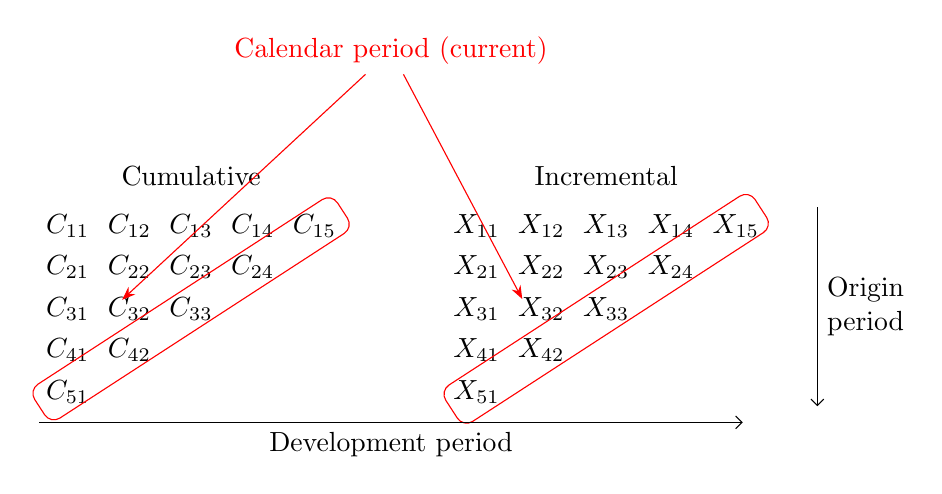
\begin{tikzpicture}[ampersand replacement=\&, LA/.style = {-Straight Barb, shorten <=1pt, shorten >=1pt,draw=black}]
    \matrix (mc) [matrix of math nodes, nodes in empty cells] {
      C_{11} \& C_{12} \& C_{13} \& C_{14} \& C_{15} \\
      C_{21} \& C_{22} \& C_{23} \& C_{24} \&        \\
      C_{31} \& C_{32} \& C_{33} \&        \&        \\
      C_{41} \& C_{42} \&        \&        \&        \\
      C_{51} \&        \&        \&        \&        \\
    };
    %
    \node[visible on=<2->, draw, rounded corners, red, inner sep=2pt, rotate fit=33, fit = (mc-5-1.west) (mc-1-5.east)] (aa) {};
    \node[left of=aa] (a) {};
    %
    \begin{scope}[xshift=150pt]
      \matrix (mx) [matrix of math nodes, nodes in empty cells] {
        X_{11} \& X_{12} \& X_{13} \& X_{14} \& X_{15} \\
        X_{21} \& X_{22} \& X_{23} \& X_{24} \&        \\
        X_{31} \& X_{32} \& X_{33} \&        \&        \\
        X_{41} \& X_{42} \&        \&        \&        \\
        X_{51} \&        \&        \&        \&        \\
      };
      \node[visible on=<2->, draw, rounded corners, red, inner sep=1pt, rotate fit=33, fit = (mx-5-1.west) (mx-1-5.east)] (bb) {};
      \node[left of=bb] (b) {};
      \draw[LA] (mc-5-1.south west |- mc.south) to node[midway, below] (temp) {Development period} (mx-5-5.south east |- mx.south);
      %
      \coordinate[right=5mm of mx.east] (e);
      \draw[LA] (mx-1-5.north east -| e) to node[midway, right, align=center] {Origin\\period} (mx-5-5.south east -| e);
      %
      \node[anchor=south] at (mc.north) {Cumulative};
      \node[anchor=south] at (mx.north) {Incremental};
      %
      \node[red, visible on=<2->] (c) at ($(temp) + (0, 5)$) {Calendar period (current)};
      \draw[red, -Stealth, visible on=<2->] (c) to (b);
      \draw[red, -Stealth, visible on=<2->] (c) to (a);
    \end{scope}
  \end{tikzpicture}
\end{frame}

\begin{frame}{Forecasting using claims triangles}
  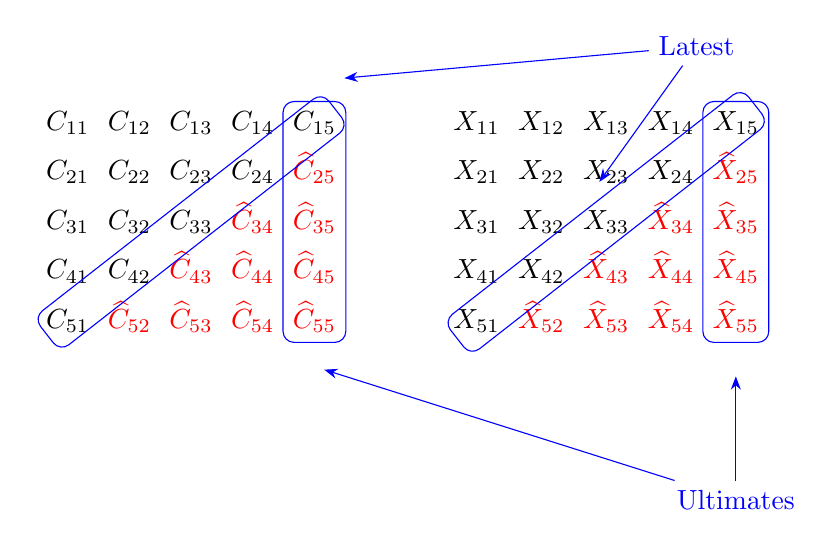
\begin{tikzpicture}[ampersand replacement=\&, LA/.style = {-Straight Barb, shorten <=1pt, shorten >=1pt,draw=black}]
    \matrix (mc) [matrix of math nodes, nodes in empty cells] {
    C_{11} \& C_{12} \& C_{13} \& C_{14} \& C_{15} \\
    C_{21} \& C_{22} \& C_{23} \& C_{24} \& |[red]| \widehat{C}_{25}  \\
    C_{31} \& C_{32} \& C_{33} \& |[red]| \widehat{C}_{34} \& |[red]| \widehat{C}_{35}  \\
    C_{41} \& C_{42} \& |[red]| \widehat{C}_{43} \& |[red]| \widehat{C}_{44} \& |[red]| \widehat{C}_{45}  \\
    C_{51} \& |[red]| \widehat{C}_{52} \& |[red]| \widehat{C}_{53} \& |[red]| \widehat{C}_{54} \& |[red]| \widehat{C}_{55}  \\
    };
    \node[visible on=<2>, draw, rounded corners, blue, inner sep=0pt, fit = (mc-1-5) (mc-5-5)] (aa) {};
    \node[below = 5pt of aa] (a) {};
    %
    \begin{scope}[xshift=150pt]
      \matrix (mx) [matrix of math nodes, nodes in empty cells] {
      X_{11} \& X_{12} \& X_{13} \& X_{14} \& X_{15} \\
      X_{21} \& X_{22} \& X_{23} \& X_{24} \& |[red]| \widehat{X}_{25}  \\
      X_{31} \& X_{32} \& X_{33} \& |[red]| \widehat{X}_{34} \& |[red]| \widehat{X}_{35}  \\
      X_{41} \& X_{42} \& |[red]| \widehat{X}_{43} \& |[red]| \widehat{X}_{44} \& |[red]| \widehat{X}_{45}  \\
      X_{51} \& |[red]| \widehat{X}_{52} \& |[red]| \widehat{X}_{53} \& |[red]| \widehat{X}_{54} \& |[red]| \widehat{X}_{55}  \\
      };
      \node[visible on=<2>, draw, rounded corners, blue, inner sep=0pt, fit = (mx-1-5) (mx-5-5)] (bb) {};
      \node[below = 5pt of bb] (b) {};
      %
      \node[blue, visible on=<2>] (c) at ($(mx-5-5.south) + (0, -2)$) {Ultimates};
      \draw[blue, -Stealth, visible on=<2>] (c) to (b);
      \draw[blue, -Stealth, visible on=<2>] (c) to (a);
      %
      \node[visible on=<3->, draw, rounded corners, blue, inner sep=0pt, rotate fit=38, fit = (mc-5-1) (mc-1-5)] (aa1) {};
      \node[above right = 1pt and 1pt of aa1] (a1) {};
      \node[visible on=<3->, draw, rounded corners, blue, inner sep=0pt, rotate fit=38, fit = (mx-5-1) (mx-1-5)] (bb1) {};
      \node[above = 1pt of bb1] (b1) {};
      \node[blue, visible on=<3->] (c1) at ($(mx-1-5.north) + (-0.5, 0.7)$) {Latest};
      \draw[blue, -Stealth, visible on=<3->] (c1) to (b1);
      \draw[blue, -Stealth, visible on=<3->] (c1) to (a1);
    \end{scope}
  \end{tikzpicture}
\end{frame}

\begin{frame}{More nomenclature}
  \begin{itemize}
    \item $I$ origin periods, $J$ development periods
    \item We assume $I = J$ (square triangles)
    \item Reserve $R = \sum_{i = 2}^I (C_{i, I} - C_{i, I + 1 - i}) = \sum_{j = 2}^I \sum_{i = I + 2 - j}^I X_{ij}$
  \end{itemize}
\end{frame}

\begin{frame}{The chain ladder}
  \begin{itemize}
    \item Most popular reserving method \footnote{According to the ASTIN 2016 Non-Life Reserving Practices Report}
    \item Originally deterministic algorithm
    \item Various attempts to frame it as a stochastic model
    \item Main assumption: there exist \emph{development factors} $f_1, \dots, f_{I - 1}$ such that
          \begin{equation*}
            \cEX{C_{ij}}{C_{i, j - 1}, \dots, C_{i1}} = f_{j - 1} C_{i, j - 1}
          \end{equation*}
  \end{itemize}
\end{frame}

\begin{frame}{Visualisation of the chain ladder}
  \begin{columns}
    \begin{column}{0.5\linewidth}
      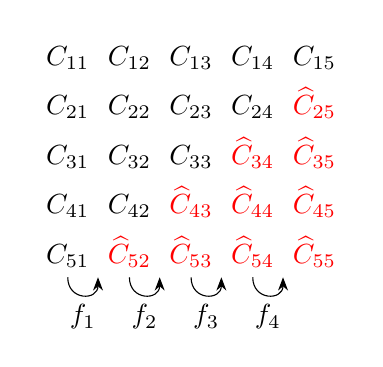
\begin{tikzpicture}[ampersand replacement=\&]
        \matrix (m) [matrix of math nodes] {
        C_{11} \& C_{12} \& C_{13} \& C_{14} \& C_{15} \\
        C_{21} \& C_{22} \& C_{23} \& C_{24} \& |[red, visible on=<5->]| \widehat{C}_{25} \\
        C_{31} \& C_{32} \& C_{33} \& |[red, visible on=<4->]| \widehat{C}_{34} \& |[red, visible on=<5->]| \widehat{C}_{35} \\
        C_{41} \& C_{42} \& |[red, visible on=<3->]| \widehat{C}_{43} \& |[red, visible on=<4->]| \widehat{C}_{44} \& |[red, visible on=<5->]| \widehat{C}_{45} \\
        C_{51} \& |[red, visible on=<2->]| \widehat{C}_{52} \& |[red, visible on=<3->]| \widehat{C}_{53} \& |[red, visible on=<4->]| \widehat{C}_{54} \& |[red, visible on=<5->]| \widehat{C}_{55} \\
        };
        \draw[-Stealth] (m-5-1.south) to [bend right, out=-90, in=-90, looseness=2] node [below] {$f_1$} (m-5-2.south west);
        \draw[-Stealth] (m-5-2.south) to [bend right, out=-90, in=-90, looseness=2] node [below] {$f_2$} (m-5-3.south west);
        \draw[-Stealth] (m-5-3.south) to [bend right, out=-90, in=-90, looseness=2] node [below] {$f_3$} (m-5-4.south west);
        \draw[-Stealth] (m-5-4.south) to [bend right, out=-90, in=-90, looseness=2] node [below] {$f_4$} (m-5-5.south west);
      \end{tikzpicture}
    \end{column}
    \begin{column}{0.5\linewidth}
      \begin{popeq}{Column sum average}
        $\displaystyle \widehat{f}_j = \frac{\sum_{i = 1}^{I - j} C_{i, j + 1}}{\sum_{i = 1}^{I - j} C_{ij}}$
      \end{popeq}
      \begin{popeq}{Chain ladder prediction}
        $\displaystyle {\widehat{C}_{ij} = C_{i, I + 1 - i} \prod_{k = I + 1 - i}^{j - 1} \widehat{f}_k}$
      \end{popeq}
    \end{column}
  \end{columns}
\end{frame}

\begin{frame}{Stochastic chain ladder}
  \begin{itemize}
    \item Many different variants
    \item Reproduce chain ladder point estimates
    \item Make different assumptions
    \item Difficult to verify with small data sizes
    \item Idea: detect violations by excluding points and gauging effect on bootstrapped reserve
  \end{itemize}
  \begin{center}
    \begin{popeq}{Normal}
      \begin{tikzpicture}[every join/.style={-Stealth}, dot/.style={circle,fill=black,inner sep=0pt, minimum size=5pt}, node distance=2mm and 1cm]
        { [start chain=trunk]
        \node[on chain, join] {Data};
        { [start branch=matrix going below]
        \node[on chain, ampersand replacement=\&, matrix of math nodes, column sep=1pt, row sep=1pt] {
        |[dot]| \& |[dot]| \& |[dot]| \& |[dot]| \& |[dot]| \\
        |[dot]| \& |[dot]| \& |[dot]| \& |[dot]| \&        \\
        |[dot]| \& |[dot]| \& |[dot]| \&         \&        \\
        |[dot]| \& |[dot]| \&         \&         \&        \\
        |[dot]| \&         \&         \&         \&        \\
        };
        }
        \node[on chain, draw, rectangle, align=center, inner sep=5pt, join] {Bootstrap};
        \node[on chain, join] {Reserve};
        { [start branch=dist going below]
        \node[on chain] {
          \begin{tikzpicture}[framed, scale=0.75]
            \draw[domain=-1:1, smooth, variable=\x] plot (\x, {exp(-0.5*(\x / 0.25)^2)});
          \end{tikzpicture}
        };
        }
        }
      \end{tikzpicture}
    \end{popeq}
  \end{center}
\end{frame}

\begin{frame}{Detecting assumption violations}
  \begin{itemize}
    \item Generate triangles which follow assumptions perfectly
    \item Apply perturbation
    \item Remove one point at a time and study impact on reserve
    \item Significant impact $\Rightarrow$ reverse-engineer
  \end{itemize}
\end{frame}


\begin{frame}{Detecting assumption violations}
  \begin{popeq}{Wrong point}
    \begin{tikzpicture}[every join/.style={-Stealth}, dot/.style={circle,fill=black,inner sep=0pt, minimum size=5pt}, node distance=2mm and 1cm]
      { [start chain=trunk]
      \node[on chain, join] {Data};
      { [start branch=matrix going below]
      \node[on chain, ampersand replacement=\&, matrix of math nodes, column sep=1pt, row sep=1pt] {
      |[at start, cross out, draw, thick, solid, blue, inner sep=2pt]| \& |[dot]| \& |[dot]| \& |[dot]| \& |[dot]| \\
      |[dot]| \& |[dot]| \& |[dot, fill=red]| \& |[dot]| \&        \\
      |[dot]| \& |[at start, cross out, draw, thick, solid, green, inner sep=2pt]| \& |[dot]| \&         \&        \\
      |[dot]| \& |[dot]| \&         \&         \&        \\
      |[dot]| \&         \&         \&         \&        \\
      };
      }
      \node[on chain, draw, rectangle, align=center, inner sep=5pt, join] {Bootstrap};
      \node[on chain, join] {Reserve};
      { [start branch=dist going below]
      \node[on chain] {
        \begin{tikzpicture}[framed, scale=0.75]
          \draw[domain=-1:1, smooth, green, variable=\x] plot (\x, {exp(-0.5*(\x / 0.25)^2)});
          \draw[domain=-1:1, smooth, blue, variable=\x] plot (\x, {exp(-0.5*((\x + 0.1) / 0.25)^2)});
        \end{tikzpicture}
      };
      }
      }
    \end{tikzpicture}
  \end{popeq}
  \begin{popeq}{Right point}
    \begin{tikzpicture}[every join/.style={-Stealth},
      dot/.style={circle,fill=black,inner sep=0pt, minimum size=5pt},
      node distance=2mm and 1cm]
      { [start chain=trunk]
      \node[on chain, join] {Data};
      { [start branch=matrix going below]
      \node[on chain, ampersand replacement=\&, matrix of math nodes, column sep=1pt, row sep=1pt] {
      |[dot]| \& |[dot]| \& |[dot]| \& |[dot]| \& |[dot]| \\
      |[dot]| \& |[dot]| \& |[at start, cross out, draw, thick, solid, red, inner sep=2pt]| \& |[dot]| \&        \\
      |[dot]| \& |[dot]| \& |[dot]| \&         \&        \\
      |[dot]| \& |[dot]| \&         \&         \&        \\
      |[dot]| \&         \&         \&         \&        \\
      };
      }
      \node[on chain, draw, rectangle, align=center, inner sep=5pt, join] {Bootstrap};
      \node[on chain, join] {Reserve};
      { [start branch=dist going below]
      \node[on chain] {
        \begin{tikzpicture}[framed, scale=0.75]
          \draw[domain=-1:1, smooth, variable=\x] plot (\x, {exp(-0.5*(\x / 0.25)^2)});
          \draw[domain=-1:1, smooth, variable=\x] plot (\x, {exp(-0.5*((\x + 0.1) / 0.25)^2)});
          \draw[domain=-1:1, smooth, red, variable=\x] plot (\x, {2.5 * (4 * (\x + 1)) * exp(-4 * (\x + 1))});
        \end{tikzpicture}
      };
      }
      }
    \end{tikzpicture}
  \end{popeq}
\end{frame}

\begin{frame}{Perturbations}
  \centering
  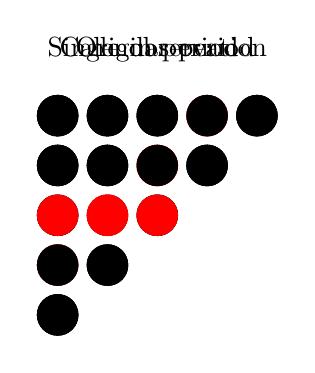
\begin{tikzpicture}
    \begin{scope}[visible on=<1>]
      \matrix[ampersand replacement=\&, matrix of math nodes, column sep=3pt, row sep=3pt, dot/.style={circle,fill=black, inner sep=0pt, minimum size=15pt}] (m) {
      |[dot]| \& |[dot]| \& |[dot]| \& |[dot]| \& |[dot]| \\
      |[dot]| \& |[dot]| \& |[dot, red]| \& |[dot]| \&        \\
      |[dot]| \& |[dot]| \& |[dot]| \&         \&        \\
      |[dot]| \& |[dot]| \&         \&         \&        \\
      |[dot]| \&         \&         \&         \&        \\
      };
      \node[above=5pt of m.north] {Single observation};
    \end{scope}
    \begin{scope}[visible on=<2>]
      \matrix[ampersand replacement=\&, matrix of math nodes, column sep=3pt, row sep=3pt, dot/.style={circle,fill=black, inner sep=0pt, minimum size=15pt}] (m) {
      |[dot]| \& |[dot]| \& |[dot]| \& |[dot, red]| \& |[dot]| \\
      |[dot]| \& |[dot]| \& |[dot, red]| \& |[dot]| \&        \\
      |[dot]| \& |[dot, red]| \& |[dot]| \&         \&        \\
      |[dot, red]| \& |[dot]| \&         \&         \&        \\
      |[dot]| \&         \&         \&         \&        \\
      };
      \node[above=5pt of m.north] {Calendar period};
    \end{scope}
    \begin{scope}[visible on=<3>]
      \matrix[ampersand replacement=\&, matrix of math nodes, column sep=3pt, row sep=3pt, dot/.style={circle,fill=black, inner sep=0pt, minimum size=15pt}] (m) {
      |[dot]| \& |[dot]| \& |[dot]| \& |[dot]| \& |[dot]| \\
      |[dot]| \& |[dot]| \& |[dot]| \& |[dot]| \&        \\
      |[dot, red]| \& |[dot, red]| \& |[dot, red]| \&         \&        \\
      |[dot]| \& |[dot]| \&         \&         \&        \\
      |[dot]| \&         \&         \&         \&        \\
      };
      \node[above=5pt of m.north] {Origin period};
    \end{scope}
  \end{tikzpicture}
\end{frame}

\section{The bootstrap method}

\begin{frame}{Main idea}
  \begin{columns}
    \begin{column}{0.5\linewidth}
      \begin{itemize}
        \item Classical inference often intractible
        \item Relies on approximations and asymptotics
        \item Solution: resampling to produce pseudo-replicates
      \end{itemize}
    \end{column}
    \begin{column}<2->{0.5\linewidth}
      \begin{figure}
        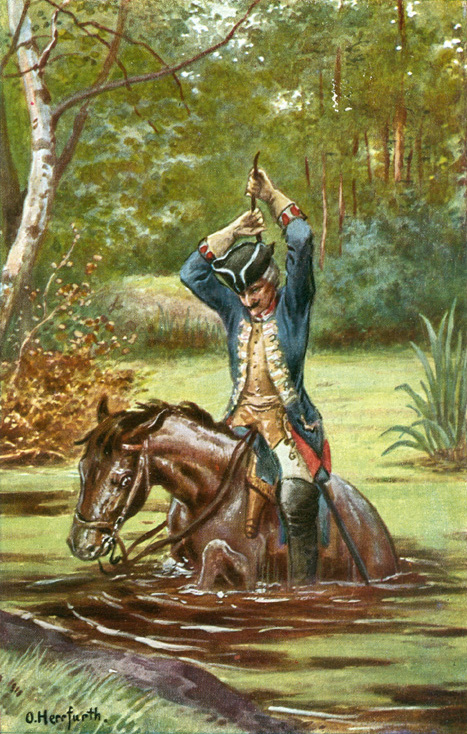
\includegraphics{munchausen.jpg}
      \end{figure}
    \end{column}
  \end{columns}
\end{frame}

\begin{frame}{Classical estimator}
  \begin{itemize}
    \item Independent identically distributed sample $X_1, \dots, X_n$
    \item Parameter $\theta$ estimated by $\widehat{\theta} \coloneqq g(X_1, \dots, X_n)$
    \item For $b = 1, \dots, B$
          \begin{itemize}
            \item Resample to obtain $X_1^{(b)}, \dots, X_n^{(b)}$
            \item Compute $\widehat{\theta}^{(b)} \coloneqq g(X_1^{(b)}, \dots, X_n^{(b)})$
            \item $\{ \widehat{\theta}^{(b)} \mid b = 1, \dots, B \}$ used for inference, e.g.\ variance estimation:
                  \begin{equation*}
                    \widehat{\mathrm{Var}}(\theta) \coloneqq \frac{1}{B - 1} \sum_{b = 1}^B (\widehat{\theta}^{(b)} - \overline{\theta}^{B})^2
                  \end{equation*}
                  with $\overline{\theta}^{B} \coloneqq \frac{1}{B} \sum_{b = 1}^B \widehat{\theta}^{(b)}$
          \end{itemize}
  \end{itemize}
\end{frame}

\begin{frame}{Parametric vs.\ nonparametric}
  \begin{itemize}
    \item How to do bootstrap resampling?
    \item Nonparametric: resample with replacement directly from data
    \item Parametric: fit model first, use this to simulate from RNG
    \item Can be extended to regression models
  \end{itemize}
\end{frame}

\begin{frame}{Regression}
  \begin{itemize}
    \item Covariates $X_1, \dots, X_p$ and response $Y$
    \item Parametrised function $f(X_1, \dots, X_p; \bm{\beta})$ modelling their relation
    \item Classic example: linear regression
          \begin{itemize}
            \item $Y_i = \bm{\mathrm{x}_i}^T \bm{\beta} + \varepsilon_i$
            \item $\EX{\varepsilon_i} = 0$, $\operatorname{Var}(\varepsilon_i) = \sigma^2$
            \item $\EX{\varepsilon_i \varepsilon_j} = 0$
            \item LS estimator: $\widehat{\bm{\beta}} \coloneqq (X^T X)^{-1} X^T \mathbf{y}$
          \end{itemize}
  \end{itemize}
\end{frame}

\begin{frame}{Regression bootstrap}
  \begin{itemize}
    \item Independent sample of predictor-response pairs $(\mathbf{x_1}, Y_1), \dots, (\mathbf{x_n}, Y_n)$
    \item For $b = 1, \dots, B$
          \begin{itemize}
            \item Resample to obtain $(\mathbf{x_1}^{(b)}, Y_1^{(b)}), \dots, (\mathbf{x_n}^{(b)}, Y_n^{(b)})$
            \item Compute $\widehat{\bm{\beta}}^{(b)}$
            \item $\{ \widehat{\bm{\beta}}^{(b)} \mid b = 1, \dots, B \}$ used for inference
          \end{itemize}
    \item Parametric vs.\ nonparametric?
  \end{itemize}
\end{frame}

\begin{frame}{Nonparametric regression bootstrap}
  \begin{itemize}
    \item Fundamental unit of resampling?
    \item Residuals $\Rightarrow$ semiparametric
    \item Pairs $\Rightarrow$ fully nonparametric
  \end{itemize}
\end{frame}

\begin{frame}{Semiparametric regression bootstrap}
  \begin{itemize}
    \item Resample residuals, e.g.
          \begin{equation*}
            r_i \coloneqq Y_i - \bm{\mathrm{x}}^T_i \widehat{\bm{\beta}}
          \end{equation*}
    \item Produce bootstrap replicates via
          \begin{equation*}
            Y_i^{(b)} \coloneqq \bm{\mathrm{x}}^T_i \widehat{\bm{\beta}} + r^{(b)}_i
          \end{equation*}
    \item Only relies on parametrisation of first two moments
  \end{itemize}
\end{frame}

\begin{frame}{Fully nonparametric regression bootstrap}
  \begin{itemize}
    \item Resample pairs to produce $(\bm{\mathrm{x}_1}^{(b)}, Y^{(b)}_1), \dots, (\bm{\mathrm{x}_n}^{(b)}, Y^{(b)}_n)$
    \item Approximates multivariate distribution of $(X_1, \dots, X_n, Y)$
    \item Model refitted to pseudo-replicates to obtain $\widehat{\bm{\beta}}^{(b)}$
    \item Does not assume anything about data (except i.i.d.-ness of sample)
  \end{itemize}
\end{frame}

\begin{frame}{Parametric regression bootstrap}
  \begin{itemize}
    \item Additional assumption about distribution of the $\varepsilon_i$
    \item Classic choice: $\varepsilon_i \sim \mathcal{N}(0, \sigma^2)$
    \item Fit model to obtain $\widehat{\bm{\beta}}$ and $\widehat{\sigma}$
    \item Produce $Y^{(b)}_i$ by drawing from the estimated distribution $\mathcal{N}(\bm{\mathrm{x}_i}^T \widehat{\bm{\beta}}, \widehat{\sigma}^2)$
    \item Relies on correct specification of parametric model
  \end{itemize}
\end{frame}

\begin{frame}{Process error}
  \begin{itemize}
    \item Methods mentioned so far produce replicates of parameter vector $\bm{\beta}$
    \item Can be used to simulate the \emph{fitted} or \emph{predicted response}
          \begin{equation*}
            \widehat{Y}^{(b)}_+ = \mathbf{x}^T_+ \widehat{\bm{\beta}}^{(b)}
          \end{equation*}
          at new value $\mathbf{x_+}$ of the regressors
    \item Incorporates estimation uncertainty or \emph{parameter error}
    \item What about simulating $Y_+$ itself?
    \item Incorporate intrinsic variation or \emph{process error}
  \end{itemize}
\end{frame}

\begin{frame}{Process error visualised}
  \centering
  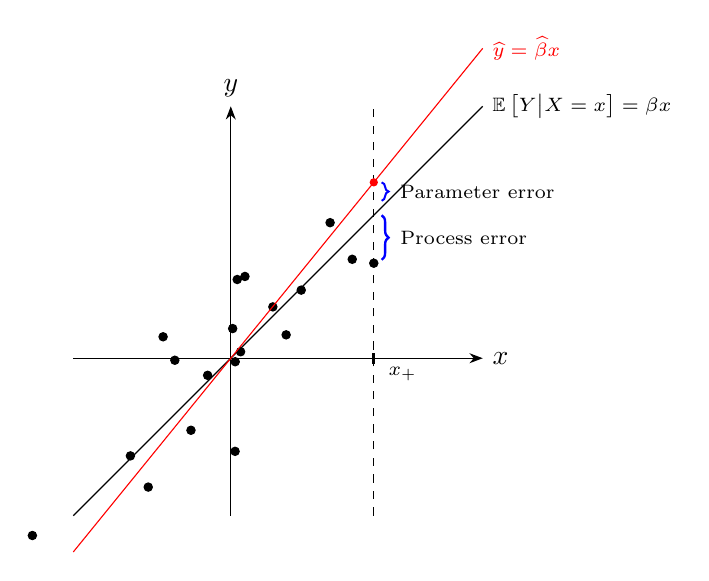
\begin{tikzpicture}
    \draw[-Stealth] (-2, 0) -- (3.2, 0) node[right] {$x$};
    \draw[-Stealth] (0, -2) -- (0, 3.2) node[above] {$y$};
    \draw[domain=-2:3.2, smooth, variable=\x] plot ({\x}, {\x}) node[right] {\scriptsize $\cEX{Y}{X = x} = \beta x$};
    %
    \draw[dashed] (1.81610604, -2) -- (1.81610604, 3.2);
    \draw[very thick] ($(1.81610604,0) + (0,-2pt)$) -- ($(1.81610604,0) + (0,2pt)$) node [below right=2pt] {\scriptsize $x_+$};
    %
    \node[draw, circle, fill=black, minimum size=3pt, inner sep=0pt] (p1) at (-0.85961786, 0.27241248) {};
    \node[draw, circle, fill=black, minimum size=3pt, inner sep=0pt] (p2) at (-1.04835062, -1.63638906) {};
    \node[draw, circle, fill=black, minimum size=3pt, inner sep=0pt] (p3) at (-0.71054275, -0.02545566) {};
    \node[draw, circle, fill=black, minimum size=3pt, inner sep=0pt] (p4) at (-1.27471311, -1.24000762) {};
    \node[draw, circle, fill=black, minimum size=3pt, inner sep=0pt] (p5) at (-2.51977736, -2.25132996) {};
    \node[draw, circle, fill=black, minimum size=3pt, inner sep=0pt] (p6) at (-0.50560237, -0.91466135) {};
    \node[draw, circle, fill=black, minimum size=3pt, inner sep=0pt] (p7) at (0.70300722, 0.29698374) {};
    \node[draw, circle, fill=black, minimum size=3pt, inner sep=0pt] (p8) at (0.05640192, -0.04435997) {};
    \node[draw, circle, fill=black, minimum size=3pt, inner sep=0pt] (p9) at (0.02398620, 0.37690827) {};
    \node[draw, circle, fill=black, minimum size=3pt, inner sep=0pt] (p10) at (-0.29417866, -0.21698233) {};
    \node[draw, circle, fill=black, minimum size=3pt, inner sep=0pt] (p11) at (1.26137046, 1.72166376) {};
    \node[draw, circle, fill=black, minimum size=3pt, inner sep=0pt] (p12) at (0.05464826, -1.18244296) {};
    \node[draw, circle, fill=black, minimum size=3pt, inner sep=0pt] (p13) at (0.17986977, 1.03857422) {};
    \node[draw, circle, fill=black, minimum size=3pt, inner sep=0pt] (p14) at (0.08175980, 0.99993873) {};
    \node[draw, circle, fill=black, minimum size=3pt, inner sep=0pt] (p15) at (1.54254771, 1.25660138) {};
    \node[draw, circle, fill=black, minimum size=3pt, inner sep=0pt] (p16) at (0.53422271, 0.65222362) {};
    \node[draw, circle, fill=black, minimum size=3pt, inner sep=0pt] (p17) at (0.12465482, 0.08242658) {};
    \node[draw, circle, fill=black, minimum size=3pt, inner sep=0pt] (p18) at (1.81610604, 1.20704277) {};
    \node[draw, circle, fill=black, minimum size=3pt, inner sep=0pt] (p19) at (0.89452603, 0.86501838) {};
    \draw[decorate, decoration={brace}, draw=blue, line width=0.3mm, transform canvas={xshift=1mm}] (1.81610604, 1.81610604) to node[right=3pt, midway, font=\scriptsize] {Process error} (1.81610604, 1.25);
    %
    \draw[domain=-2:3.2, smooth, red, variable=\x] plot ({\x}, {1.23*\x}) node[right] {\scriptsize $\widehat{y} = \widehat{\beta} x$};
    \node[draw, circle, fill=red, draw=none, minimum size=3pt, inner sep=0pt] (p20) at (1.81610604, 2.23381) {};
    \draw[decorate, decoration={brace}, draw=blue, line width=0.25mm, transform canvas={xshift=1mm}] (1.81610604, 2.23381) to node[right=3pt, midway, font=\scriptsize] {Parameter error} (1.81610604, 2);
  \end{tikzpicture}
\end{frame}


\begin{frame}{Predictive distribution}
  \begin{itemize}
    \item Bayesian concept
    \item Incorporates both parameter and process error
    \item Semiparametric: resample residuals a second time and compute
          \begin{equation*}
            Y_+^{(b, s)} \coloneqq \mathbf{x}_+^T \widehat{\bm{\beta}}^{(b)} + r^{(s)}
          \end{equation*}
    \item Parametric: generate pseudo-response according to
          \begin{equation*}
            Y^{(b, s)}_+ \sim \mathcal{N}(\mathbf{x}^T_+ \widehat{\bm{\beta}}^{(b)}, \widehat{\sigma}^2)
          \end{equation*}
    \item Nonparametric: borrow one of the other approaches
  \end{itemize}
\end{frame}

\section{Mack's model}

\begin{frame}{Formulation}
  \small
  \begin{model}[Mack chain ladder]
    \begin{enumerate}
      \item There exist development factors $f_1, \dots, f_{I - 1}$ such that
            \begin{equation*}
              \mathbb{E}[C_{ij} \ \Vert \ C_{i, j - 1}, \dots, C_{i1}] = \mathbb{E}[C_{ij} \ \Vert \ C_{i, j - 1}] = f_{j - 1} C_{i, j - 1}
            \end{equation*}
            for $1 \leq i \leq I$
      \item There exist variance parameters $\sigma_1, \dots, \sigma_{I - 1}$ such that
            \begin{equation*}
              \mathrm{Var}[C_{ij} \ \Vert \ C_{i, j - 1}, \dots, C_{i1}] = \mathrm{Var}[C_{ij} \ \Vert \ C_{i, j - 1}] = \sigma_{j - 1}^2 C_{i, j - 1}
            \end{equation*}
            for $1 \leq i \leq I$
      \item The cumulative claims processes $(C_{ij})_j, (C_{i'j})_j$ are independent for $i \neq i'$
    \end{enumerate}
  \end{model}
\end{frame}

\begin{frame}{Properties}
  \begin{itemize}
    \item Cumulative triangle
    \item Distribution-free
    \item Recursive
    \item For any pair of consecutive columns: equivalent to
          \begin{equation*}
            \bm{\mathrm{c}_{j + 1}} = f_j \bm{\mathrm{c}_j} + \bm{\varepsilon}
          \end{equation*}
          with
          \begin{align*}
            \cEX{\bm{\varepsilon}}{C_{1, j}, \dots, C_{I - j, j}}   & = \bm{0}     \\
            \cVarX{\bm{\varepsilon}}{C_{1, j}, \dots, C_{I - j, j}} & = \sigma^2_j
            \begin{bmatrix}
              C_{1j} &        &              \\
                     & \ddots &              \\
                     &        & C_{I - j, j}
            \end{bmatrix}
          \end{align*}
  \end{itemize}
\end{frame}

\begin{frame}{Properties}
  \begin{itemize}
    \item Model assumptions correspond to Gauss-Markov
    \item Optimal estimator: weighted least squares with
          \begin{equation*}
            \mathbf{W} =
            \begin{bmatrix}
              1 / C_{1j} &        &                  \\
                         & \ddots &                  \\
                         &        & 1 / C_{I - j, j}
            \end{bmatrix}
          \end{equation*}
    \item Same as column sum estimator!
          \begin{equation*}
            \widehat{f}^{\mathrm{WLS}}_j = (\bm{\mathrm{c}_j}^T \mathbf{W} \bm{\mathrm{c}_j})^{-1} \bm{\mathrm{c}_j}^T \mathbf{W} = \frac{\sum_{i = 1}^{I - j} C_{i, j + 1}}{\sum_{i = 1}^{I - j} C_{i, j}}
          \end{equation*}
    \item We can adapt the regression bootstrap!
  \end{itemize}
\end{frame}

\begin{frame}{Conditional vs.\ unconditional}
  \begin{itemize}
    \item Recursivity leads to different bootstrap types
    \item Simulate next development year based on original data vs.\ generated bootstrap replicate
    \item Parametric example:
          \begin{equation*}
            C^{(b)}_{i, j + 1} \sim \mathcal{N}(\widehat{f}_j C_{ij}, \widehat{\sigma}^2_j) \quad \text{vs.} \quad C^{(b)}_{i, j + 1} \sim \mathcal{N}(\widehat{f}_j C^{(b)}_{ij}, \widehat{\sigma}^2_j)
          \end{equation*}
  \end{itemize}
\end{frame}

\begin{frame}{Wealth of configurations}
  \begin{itemize}
    \item Conditional vs.\ unconditional
    \item Nonparametric: only conditional is possible!
    \item Parametric: which distribution?
          \begin{itemize}
            \item Normal
            \item Gamma
          \end{itemize}
    \item Semiparametric: which residuals?
          \begin{itemize}
            \item Standardised
            \item Studentised
            \item Log-normal
          \end{itemize}
    \item Computationally very intensive!
  \end{itemize}
\end{frame}

\begin{frame}[label=implementation]{Implementation}
  \begin{itemize}
    \item R package \texttt{claimsBoot}
    \item Front-end in R
    \item Heavy-duty numerical code in Fortran
    \item Parallelised using OpenMP
    \item Glued together with \texttt{Rcpp}
    \item Available on Github
  \end{itemize}
\end{frame}

\begin{frame}{Results}
  \begin{itemize}
    \item Parametric
          \begin{itemize}
            \item Good performance
            \item Unconditional better than conditional
          \end{itemize}
    \item Semiparametric
          \begin{itemize}
            \item Standardised \& log-normal residuals yield bad results
            \item Studentised residuals do reasonably well
          \end{itemize}
    \item Nonparametric
          \begin{itemize}
            \item Performance in-between parametric/studentised and standardised/log-normal
          \end{itemize}
    \item Differences more noticeable closer to current calendar period
    \item For calendar \& origin outliers: same trends, more pronounced
    % \item Visualisation: Shiny app
  \end{itemize}
\end{frame}

\section{The ODP model}

\begin{frame}{Formulation}
  \begin{model}[overdispersed Poisson GLM]
    \begin{enumerate}
      \item The incremental claims are independent from each other
      \item There exist parameters $c$, $a_1, \dots, a_I$ and $b_1, \dots, b_I$ such that
            \begin{equation*}
              \log(\mu_{ij}) = c + a_i + b_j
            \end{equation*}
            with $\mu_{ij} \coloneqq \EX{X_{ij}}$ and $a_1 = b_1 = 0$
      \item There exists a parameter $\phi$ such that
            \begin{equation*}
              \VarX{X_{ij}} = \phi \mu_{ij}
            \end{equation*}
    \end{enumerate}
  \end{model}
\end{frame}

\begin{frame}{Properties}
  \begin{itemize}
    \item Incremental triangle
    \item Belongs to family of \emph{generalised linear models}
          \begin{itemize}
            \item Extend normal linear model
            \item Response can follow any distribution from the EDM family
            \item Covariates related to response via \emph{link function}
          \end{itemize}
    \item Dispersion parameter allowing mean to differ from variance (cfr.\ Poisson)
    \item Fitted using quasi-maximum likelihood
    \item Equations solved iteratively using Fisher scoring
  \end{itemize}
\end{frame}

\begin{frame}{Triangle to regression}
  \begin{columns}
    \begin{column}{0.5\linewidth}
      \begin{itemize}
        \item Flatten triangle to obtain regression model
        \item Development and origin year become the covariates
        \item Cfr.\ two-way ANOVA (without interaction)
        \item We can adapt the regression bootstrap!
      \end{itemize}
    \end{column}
    \begin{column}<2->{0.5\linewidth}
      \centering
      \resizebox*{!}{0.7\textheight}{%
        \begin{tabular}{ccc}\toprule%
          \bf{Origin} & \bf{Dev} & \bf{Value} \\ \midrule
          \csvreader[
          late after line =                   \\,
            range = 1-15
          ]{%
            UKMotor_long.csv
          }{origin=\Origin, dev=\Dev, value=\Value}{%
          \Origin     & \Dev     & \Value
          }\bottomrule%
        \end{tabular}
      }
    \end{column}
  \end{columns}
\end{frame}

\begin{frame}{Triangle to regression}
  \begin{tikzpicture}[transform canvas={scale=0.8}, xshift=85pt, yshift=50pt]
    \matrix (m) [ampersand replacement=\&, matrix of math nodes] {
      X_{11} \& X_{12} \& X_{13} \& X_{14} \& X_{15} \\
      X_{21} \& X_{22} \& X_{23} \& X_{24}           \\
      X_{31} \& X_{32} \& X_{33}                     \\
      X_{41} \& X_{42}                               \\
      X_{51}                                         \\
    };
    \draw[-Stealth] (m-1-1.north west) -- ++(-0.5, 0.5) node[above, blue] {$c$};
    %
    \draw[-Stealth] (m-1-2.north) -- ++(0, 0.5) node[above, red] {$b_2$};
    \draw[-Stealth] (m-1-3.north) -- ++(0, 0.5) node[above, red] {$b_3$};
    \draw[-Stealth] (m-1-4.north) -- ++(0, 0.5) node[above, red] {$b_4$};
    \draw[-Stealth] (m-1-5.north) -- ++(0, 0.5) node[above, red] {$b_5$};
    %
    \draw[-Stealth] (m-2-1.west) -- ++(-0.5, 0) node[left, green] {$a_2$};
    \draw[-Stealth] (m-3-1.west) -- ++(-0.5, 0) node[left, green] {$a_3$};
    \draw[-Stealth] (m-4-1.west) -- ++(-0.5, 0) node[left, green] {$a_4$};
    \draw[-Stealth] (m-5-1.west) -- ++(-0.5, 0) node[left, green] {$a_5$};
    \matrix (mm) [below right=0.1cm and 0.5cm of m, ampersand replacement=\&, matrix of math nodes, nodes in empty cells, left delimiter={[}, right delimiter={]},
        column 1/.style = {blue},
        column 2/.style = {green},
        column 3/.style = {green},
        column 5/.style = {red},
      ] {
        1 \& 0 \& 0 \& \hdots \& 0 \\
        1 \& 1 \& 0 \& \hdots \& 0 \\
        1 \& 0 \& 1 \& \hdots \& 0 \\
        \vdots \& \vdots \& \vdots \& \ddots \& \vdots \\
        1 \& 0 \& 0 \& \hdots \& 1 \\
      };
    \matrix (mv) [
    right=0.5 of mm,
    ampersand replacement=\&, matrix of math nodes, nodes in empty cells, left delimiter={[}, right delimiter={]}] {
    |[blue]| c \\ |[green]| a_2 \\ |[green]| a_3 \\ \vdots \\ |[red]| b_5 \\
    };
    \node (eq) [right=0.5 of mv] {$=$};
    \matrix (mvv) [
    right=0.5 of eq,
    ampersand replacement=\&, matrix of math nodes, nodes in empty cells, left delimiter={[}, right delimiter={]}] {
        \log(\mu_{11}) \\ \log(\mu_{21}) \\ \log(\mu_{31}) \\ \vdots \\ \log(\mu_{15}) \\
      };
    \draw[-Stealth, bend left, very thick] (m.east) -| (mm.north);
  \end{tikzpicture}
\end{frame}

\begin{frame}{Configurations}
  \begin{itemize}
    \item Parametric: which distribution?
          \begin{itemize}
            \item Normal
            \item Gamma
            \item Poisson
          \end{itemize}
    \item Semiparametric: which residuals?
          \begin{itemize}
            \item Most popular ones for GLM: Pearson and deviance
            \item Deviance suffer technical shortcoming which inhibits resampling
          \end{itemize}
    \item Nonparametric: impossible
    \item Computationally very intensive!
  \end{itemize}
\end{frame}

\againframe{implementation}

\begin{frame}{Results}
  \begin{itemize}
    \item Parametric outperforms semiparametric
    \item Differences more noticeable closer to current calendar period
    \item For calendar \& origin outliers: same trends, more pronounced
    % \item Visualisation: Shiny app
  \end{itemize}
\end{frame}

\section{Conclusion}

\begin{frame}{Key takeaways}
  \begin{itemize}
    \item Parametric bootstraps perform very well
    \item For semiparametric bootstraps, result depends on residuals
    \item For Mack's model: nonparametric bootstrap performs reasonably well, but outclassed by parametric variant
    \item Flag suspicious datapoints by reverse-engineering the simulation process
  \end{itemize}
\end{frame}

\begin{frame}{Future research}
  \begin{itemize}
    \item Other types of deviations
    \item Robust methods in semiparametric bootstrap
  \end{itemize}
\end{frame}

\end{document}